\chapter{Pipelining}

\section{What is Pipelining?}
Pipeline is a technique used in CPUs to execute multiple instructions simultaneously by breaking the instruction execution process into stages.

\vspace{-\baselineskip}
\begin{figure}[H]
\centering
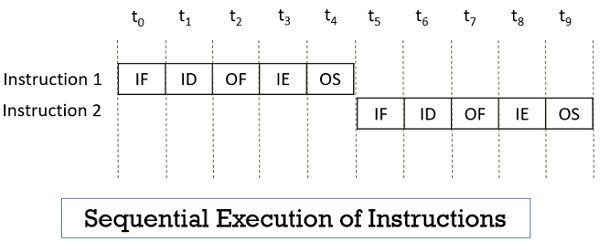
\includegraphics[width=0.45\textwidth]{figures/Non-pipelined.png}
\hfill
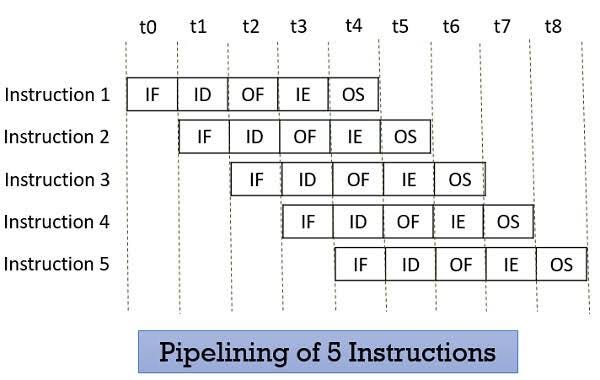
\includegraphics[width=0.45\textwidth]{figures/Pipelined.png}
\end{figure}

\subsubsection{Typical stages in a CPU pipeline:}
\begin{itemize}[parsep=0.5em]
   \item Fetch (IF) - Get the instruction from memory.
   \item Decode (ID) - Determine what the instruction does.
   \item Execute (EX) - Perform the operation (e.g., ALU computation).
   \item Memory Access (MEM) - Read/write data from/to memory.
   \item Write Back (WB) - Store the result back to a register.
\end{itemize}

\subsubsection{Benefits of Pipelining:}
\begin{itemize}[parsep=0.5em]
   \item Increased throughput:
   Multiple instructions are in progress at the same time — so more instructions complete per second.
   \item Efficient use of CPU:
   All parts of the CPU stay busy doing specific tasks in parallel.
   \item Faster instruction processing for workloads:
   Especially when executing many instructions — like in loops or large programs.
\end{itemize}

% \subsubsection{Challenges in Pipelining:}
% \begin{itemize}[parsep=0.5em]
%    \item Pipeline hazards:
%    \item Data hazards:
%    \item Control hazards:
% \end{itemize}
